
\section{Data Description}

Existing IKGQA datasets often simulate incompleteness by removing triples from gold relation paths, as illustrated in Figure~\ref{fig:IKG_Construction}(a). To better capture real-world KG dynamics, we construct IKGWQ by revisiting samples from CWQ and WebQSP and rebuilding corresponding question-answer using up-to-date knowledge, as shown in Figure~\ref{fig:IKG_Construction}(b).

\begin{figure}[t]
    \centering
    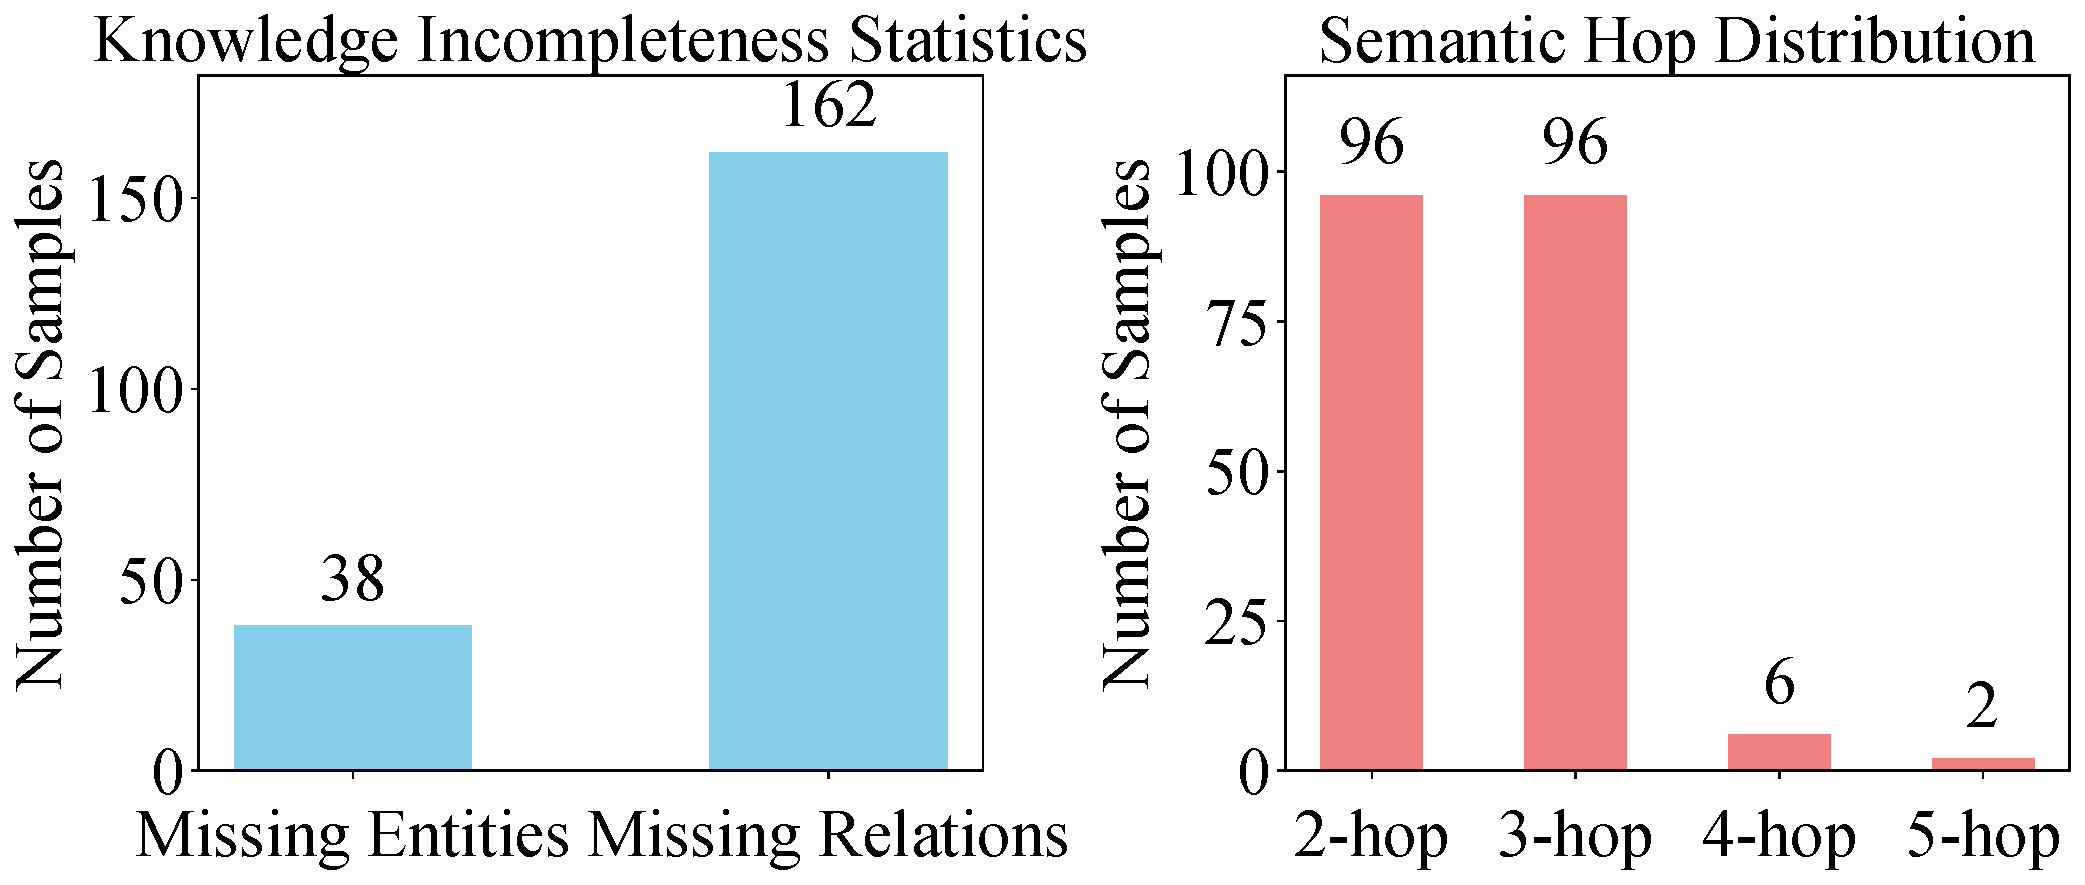
\includegraphics[width=\linewidth]{figures/figure_11.pdf}
    \caption{Statistics of knowledge incompleteness and semantic hop distribution in the IKGWQ dataset. The left subfigure shows the number of samples with missing entities and missing relations. The right subfigure presents the distribution of semantic inference hops.}
    \label{fig:dataset_analysis}
\end{figure}

Specifically, we revisit each selected sample by retrieving up-to-date information for its topic entity from reliable sources and constructing question-answer pairs that reflect facts missing or outdated in the original Freebase~\cite{bollacker2008freebase} KG.  First, we extract topic entities from the original datasets and retrieve their updated descriptions via the Wikipedia API. We then guide an LLM to generate question-answer pairs based on knowledge extracted from these texts—focusing particularly on facts beyond the scope of the original KG. Finally, we conduct manual filtering, question rewriting, and human annotation to ensure the quality and correctness of the resulting dataset. This pipeline naturally introduces both missing triples and missing entities, offering a more realistic simulation of the dynamic and uncertain nature of KG incompleteness in real-world scenarios.



To better understand the characteristics and challenges posed by the IKGWQ dataset, we conduct a detailed analysis in two key dimensions: knowledge incompleteness and inference complexity. The results are summarized in Figure~\ref{fig:dataset_analysis}. The dataset comprises 200 samples, including 38 instances of missing entities and 162 instances of missing relations. Note that missing-entity cases inherently subsume relation incompleteness, whereas missing-relation cases do not involve any entity omission. In terms of inference complexity, a substantial portion of questions require multi-hop inference: 48\% of the samples involve 3-hop inference, with some extending up to 5-hop. Note that hop count is defined based on the number of semantic inference steps needed to answer a question, excluding auxiliary nodes such as Compound Value Type nodes in Freebase. The actual KG traversal steps may be higher due to these intermediate structures.